%=========================================================================
% Start of
%=========================================================================
\preClass{Operations on Functions}

\begin{problem}
\item A restaurant would like to test a new menu item. They estimate
  that the cost for producing $x$ servings in market A is 12\$ per
  serving. They estimate that the cost for producing $y$ servings in
  market B is \$15 per serving.  They will allocate a total of
  \$36,000 for producing the total number of servings. Write out an
  expression that relates the cost of the number of servings produced
  in market A and market B.
  \vfill
\item The number of mosquitoes per acre in an area is estimated to be
  600 times the area of open water measured in acres. The area of open
  water in a location is declining over time and is
  $A(t)=50-\frac{1}{3}t$, where $t$ is the number of years since
  January 1 of the current year. Determine the number of mosquitoes
  per acre in terms of $t$.
  \vfill
\item The delay time required for a neuron to recharge is estimate to
  be a function of the calcium concentration,
  \begin{eqnarray*}
    \mathrm{Recharge([Ca])} & = & 0.05-\mathrm{[Ca]}^2.
  \end{eqnarray*}
  The concentration of calcium in an experiment is changed over time
  and is estimated to be
  \begin{eqnarray*}
    \mathrm{[Ca]}(t) & = & 0.01+\frac{1}{1+t}.
  \end{eqnarray*}
  Determine the formula used to estimate the recharge delay as a
  function of time, $t$. \textit{(Do not simplify the expression.)}
  \vfill
\end{problem}


\actTitle{Operations on Functions}
\begin{problem}
\item A function is defined to be
  \begin{eqnarray*}
    f(x) & = & x^2.
  \end{eqnarray*}
  Determine the value of $a$ and $b$ so that the function
  \begin{eqnarray*}
    g(x) & = & f(x-a)+b
  \end{eqnarray*}
  is the original function that is shifted up two units and left 3
  units. Plot the graphs of $f(x)$ and $g(x)$ on the coordinate plane below.

  \begin{tikzpicture}[y=1.1cm, x=1.1cm,font=\sffamily]
      % bounds
      \def\lowX{-5.5}
      \pgfmathtruncatemacro\startX{round(0.5+\lowX)}
      \pgfmathsetmacro\nextXValue{int(\startX+1)}
      \def\highX{5.5}
      \def\lowY{-5.5}
      \def\highY{5.5}
      \pgfmathsetmacro\nextYValue{int(\lowY+1)}
      % ticks
      \draw[step = 1, gray, very thin,dashed,opacity=0.85] (\lowX, \lowY) grid ( \highX,\highY);
    % axis
    \draw[thick,->] (\lowX,0) -- coordinate (x axis mid) (\highX,0) node[anchor = north west] {$x$};
      \draw[thick,->] (0,\lowY) -- coordinate (y axis mid) (0,\highY) node[anchor = north east] {$y$};
      \foreach \y in {-5,-4,...,-1,1,2,...,\highY} {
        \draw (1pt, \y) -- (-1pt, \y) node[yshift=-6,xshift=-1,anchor=east] {$\y$};
      }
      \foreach \x in {-5,-4,...,-1,1,2,...,\highX} {
        \draw (\x,1pt) -- (\x,-1pt) node[yshift=-5,xshift=-1,anchor=east] {$\x$};
      }
      \draw (0,5.5) node [anchor=south] {Comparing Shifted Functions};
    \end{tikzpicture}

  \clearpage

\item Two functions are given in the tables below.

  \begin{tabular}[h]{l||l|l|l|l|l}
    $x$    & 0 & 1 & 2 & 3 & 4 \\ \hline
    $f(x)$ & a & m & k & a & h \\
  \end{tabular}

  \begin{tabular}[h]{l||l|l|l|l|l}
    $x$    & a & c & h & j & m \\ \hline
    $g(x)$ & $\natural$ & $\Diamond$ & $\Box$ & $\heartsuit$ & $\Diamond$ \\
  \end{tabular}

  \begin{subproblem}
  \item Determine the range and domain of $f$.
    \vspace{2em}
  \item Determine the range and domain of $g$.
    \vspace{2em}
  \item Determine the values of each of the following expressions:
    \begin{eqnarray*}
      f(2) & = & \\
      f(4) & = & \\
      g(f(2)) & = & \\
      g(f(1)) & = & \\
      g(f(0))+g(f(3)) & = &
    \end{eqnarray*}
  \item If $f(x)=$h what is the value of $x$?
  \end{subproblem}

  \clearpage

\end{problem}

\postClass

\begin{problem}
\item Briefly state two ideas from today's class.
  \begin{itemize}
  \item
  \item
  \end{itemize}

\item Two functions are given in the tables below.

  \begin{tabular}[h]{l||l|l|l|l|l}
    $x$    & 0 & 1 & 2 & 3 & 4 \\ \hline
    $f(x)$ & a & m & k & a & h \\
  \end{tabular}

  \begin{tabular}[h]{l||l|l|l|l|l}
    $x$    & a & c & h & j & m \\ \hline
    $g(x)$ & $\natural$ & $\Diamond$ & $\Box$ & $\heartsuit$ & $\Diamond$ \\
  \end{tabular}

  \begin{subproblem}
  \item If $g(f(x))=\natural$ what are the possible values of $x$? Is
    this reverse procedure a function?
  \item If $g(x)=\Diamond$ what are the possible values of $x$? Is
    this reverse procedure a function?
  \item Express the function $g(f(x))$ as a table.
  \item Determine the range and domain of $g(f(x))$.
  \end{subproblem}

  \clearpage

\item Two functions are shown in the figure below. The function
  plotted with the dotted line is $f(x)$, and the function plotted
  with the solid line is $g(x)$. Express $g(x)$ in terms of $f(x)$,
  \begin{eqnarray*}
    g(x) & = &
  \end{eqnarray*} \\
  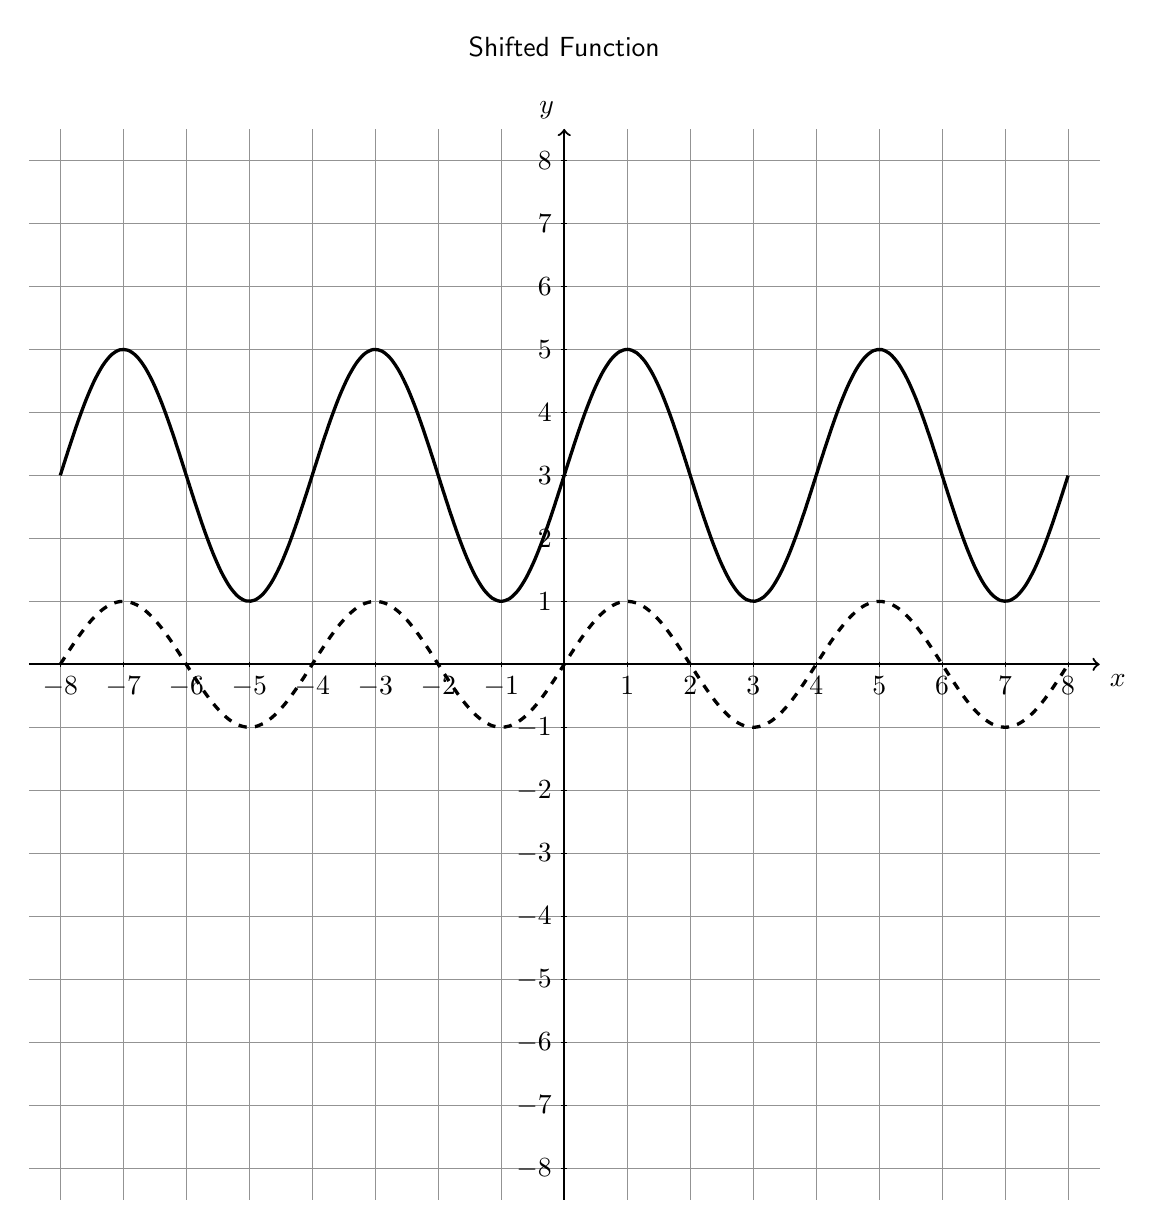
\begin{tikzpicture}[y=0.8cm, x=0.8cm,font=\sffamily]
  % Define the x bounds
  \def\lowX{-8.5}
  \pgfmathtruncatemacro\startX{round(0.5+\lowX)}
  \def\highX{8.5}
  \pgfmathtruncatemacro\endX{round(\highX-0.5)}
  % define the y bounds
  \def\lowY{-8.5}
  \pgfmathtruncatemacro\startY{round(0.5+\lowY)}
  \def\highY{8.5}
  \pgfmathtruncatemacro\endY{round(\highY-0.5)}
  % Add a grid
  \draw[step = 1, gray, very thin,opacity=0.85] (\lowX, \lowY) grid ( \highX, \highY);
% Draw the axes
\draw[thick,->] (\lowX,0) -- coordinate (x axis mid) (\highX,0) node[anchor = north west] {$x$};
  \draw[thick,->] (0,\lowY) -- coordinate (y axis mid) (0,\highY) node[anchor = south east] {$y$};
  % Label the y axis
  \pgfmathsetmacro\nextYValue{int(\startY+1)}
  \foreach \y in {\startY,\nextYValue,...,-1,1,2,...,\highY} {
    \draw (1pt, \y) -- (-1pt, \y) node[anchor = east] {$\y$};
  }
  % Label the x axis
  \pgfmathsetmacro\nextXValue{int(\startX+1)}
  \foreach \x in {\startX,\nextXValue,...,-1,1,2,...,\endX} {
    \draw (\x,1pt) -- (\x,-1pt) node[anchor = north] {$\x$};
  }
  % Draw the function.
  \begin{scope}
    %\clip(-4,-1) rectangle (8,5);
    \draw[scale=1.0,domain=\startX:\endX,smooth,variable=\x,very thick,black,samples=120]
         plot ({\x},{3+2*sin(deg(pi*\x/2))});
     \draw[scale=1.0,domain=\startX:\endX,smooth,variable=\x,very thick,dashed,black,samples=120]
        plot ({\x},{sin(deg(pi*\x/2))});
  \end{scope}

  %\node[above=0.1cm] at (-2,2 )   {\nextXValue};
  \draw (0,9.5) node [anchor=south] {Shifted Function};

\end{tikzpicture}

\clearpage

\item Two functions are shown in the figure below. The function
  plotted with the dotted line is $f(x)$, and the function plotted
  with the solid line is $g(x)$. Express $g(x)$ in terms of $f(x)$.
  \begin{eqnarray*}
    g(x) & = &
  \end{eqnarray*} \\
  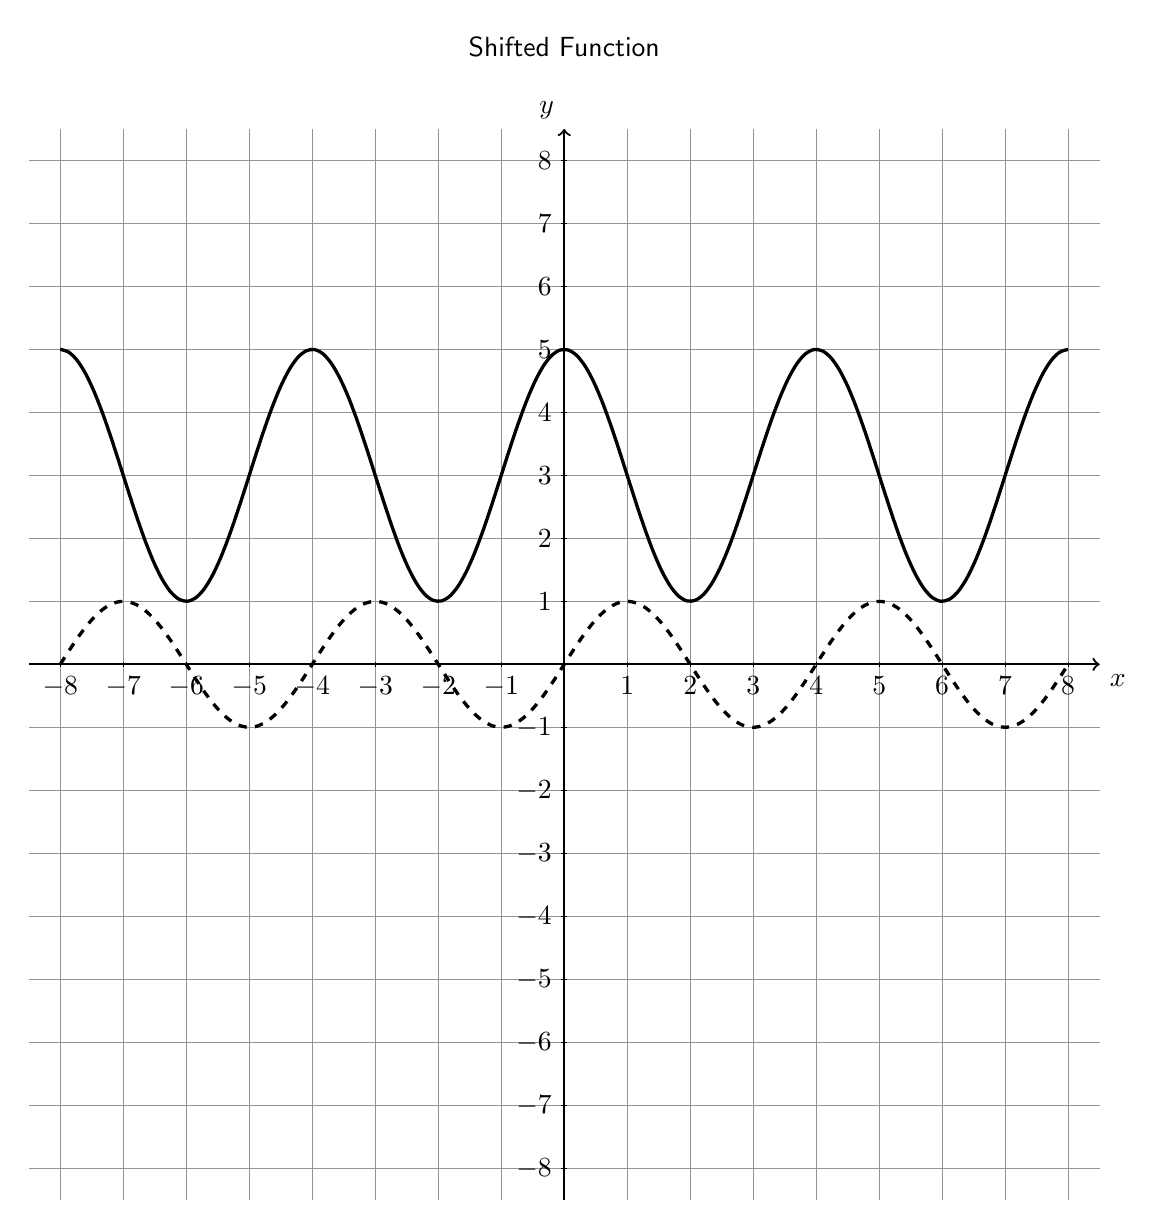
\begin{tikzpicture}[y=0.8cm, x=0.8cm,font=\sffamily]
  % Define the x bounds
  \def\lowX{-8.5}
  \pgfmathtruncatemacro\startX{round(0.5+\lowX)}
  \def\highX{8.5}
  \pgfmathtruncatemacro\endX{round(\highX-0.5)}
  % define the y bounds
  \def\lowY{-8.5}
  \pgfmathtruncatemacro\startY{round(0.5+\lowY)}
  \def\highY{8.5}
  \pgfmathtruncatemacro\endY{round(\highY-0.5)}
  % Add a grid
  \draw[step = 1, gray, very thin,opacity=0.85] (\lowX, \lowY) grid ( \highX, \highY);
% Draw the axes
\draw[thick,->] (\lowX,0) -- coordinate (x axis mid) (\highX,0) node[anchor = north west] {$x$};
  \draw[thick,->] (0,\lowY) -- coordinate (y axis mid) (0,\highY) node[anchor = south east] {$y$};
  % Label the y axis
  \pgfmathsetmacro\nextYValue{int(\startY+1)}
  \foreach \y in {\startY,\nextYValue,...,-1,1,2,...,\highY} {
    \draw (1pt, \y) -- (-1pt, \y) node[anchor = east] {$\y$};
  }
  % Label the x axis
  \pgfmathsetmacro\nextXValue{int(\startX+1)}
  \foreach \x in {\startX,\nextXValue,...,-1,1,2,...,\endX} {
    \draw (\x,1pt) -- (\x,-1pt) node[anchor = north] {$\x$};
  }
  % Draw the function.
  \begin{scope}
    %\clip(-4,-1) rectangle (8,5);
    \draw[scale=1.0,domain=\startX:\endX,smooth,variable=\x,very thick,black,samples=120]
         plot ({\x},{3+2*sin(deg(pi*\x/2+pi/2))});
     \draw[scale=1.0,domain=\startX:\endX,smooth,variable=\x,very thick,dashed,black,samples=120]
        plot ({\x},{sin(deg(pi*\x/2))});
  \end{scope}

  %\node[above=0.1cm] at (-2,2 )   {\nextXValue};
  \draw (0,9.5) node [anchor=south] {Shifted Function};

\end{tikzpicture}

  Add a sketch of the graph of the function $h(x)=3f(x+2)-5$ to the plot above.

  Can you find a different formula whose graph looks exactly the same as $g(x)$?


\end{problem}


%%% Local Variables:
%%% mode: latex
%%% TeX-master: "../labManual"
%%% End:
